%&LaTeX

\documentclass[a4paper,12pt,man]{apa} % nobf, doc, apa

\usepackage[]{amsmath, amsfonts, amstext, amsthm} 
\usepackage{amssymb}
\usepackage[]{graphics} 
\usepackage{graphicx} 
\usepackage{epsfig}
\usepackage{epstopdf}

\newcommand{\citep}{\cite} 
\newcommand{\citet}{\citeA}
\newcommand{\mat}{\mathbf} 
\newcommand{\vc}{\mathbf}

\newcommand{\pkg}{\texttt}
\newcommand{\code}{\texttt}

\renewcommand{\baselinestretch}{2}

\title{A Framework for Discrete Change}

\author{Ingmar Visser \& Maarten Speekenbrink}

\date{\today}

\affiliation{Department of Psychology, University of Amsterdam\\
 Correspondence concerning this article should be addressed to:
 \\
 Ingmar Visser \\
 Department of Psychology, University of Amsterdam \\
 Roetersstraat 15 \\
 1018 WB Amsterdam \\
 phone: +31 (20) 5256723 \\
 fax: +31 (20) 6390279 \\
 email: i.visser@uva.nl}
 
 
\shorttitle{Modelling Discrete Change}
 
\abstract{A class of models is developed for measuring and detecting
discrete change in learning and development.  The basic model for
detecting such change is the latent or hidden Markov model.
Traditionally, these models were restricted to categorical, mostly
binary, observed variables, placing severe restrictions on possible
measurement models.  In this paper, the basic model is extended to
include arbitrary distributions for the observed variables, including
multi-variate distributions.  Moreover, there is optional support to
include time-varying predictors.  In effect, this model consists of
mixtures of general linear models with Markovian depencies over time
to model the change process.  In addition, transition parameters can
be made to depend on covariates as well, such that the switching
regime between states depends on characteristics of the individual or
the experimental situation.  The model is illustrated with an example
of participants' learning in the weather prediction task.}
    
  
\begin{document}
\maketitle

% intro
Discrete change frequently occurs in learning and development: in
learning concepts, in performance on Piagetian tasks, in
discrimination learning and in conditioning.  This chapter is
concerned with detecting the time points of change in (individual)
time series.  We present a framework of dependent mixture models that can
be used to differentiate between gradual and discrete learning events
in individual time series data.  Before presenting the model in formal
terms and providing some illustrations, we first review some examples
in which discrete change is found.

% phenomena of discrete change in development/learning
Piagetian developmental theory (REFERENCE??)  assumes step-wise
changes in the strategies that children apply in all kinds of tasks
such as the conservation learning and the balance scale task.  Van der
Maas et al.  (1992) developed a catastrophe model to describe phase
transitions in learning and developmental processes.  They applied the
catastrophe model to learning in the conservation of liquid task
(REFERENCE??)  in which children have to judge relative volumes of
liquid in glasses of different heights and widths.  Young children
tend to ignore the width dimension and hence always choose the glass
with the highest level of liquid (REFERENCE??).  Van der Maas et al.
(1992) showed that there is a sudden transition to a new strategy in
which the children also take the width of the glasses into account
when judging the volume of liquids.

% balance scale rules
Jansen and Van der Maas (2001) applied the catastrophe model to
development of strategies on the balance scale task (Siegler, 1981).
In the balance scale task participants have to judge which side of a
balance goes down when the number of weights and their distances to
the fulcrum are varied over trials.  Younger children tend to ignore
the distance dimension in this task, and instead focus solely on the
number of weights on each side of the fulcrum.  This strategy for
solving balance scale items is called Rule 1 (Siegler, 1981).  Older
children include the distance dimension in determining their response
to balance scale problems; however, they only do so when the weight
dimension does not differ between the sides of the balance, i.e., when
the number of weights is equal on both sides of the balance scale.
This strategy is called Rule 2 (Siegler, 1981).

% hysteresis on the balance scale
Jansen and Van der Maas (2001) found clear evidence for stage-wise
transitions between Rule 1 and Rule 2 by testing criteria that were
derived from the catastrophe model.  In particular, they found bimodal
test scores and inaccessibility.  The latter means that there are no
in-between strategies: children apply either Rule 1 or Rule 2 and
there is no in-between option.  Jansen and Van der Maas also found
evidence for hysteresis: the phenomenon that switching between
strategies is assymetric.  Children can switch from Rule 1 to Rule 2
and back, but this occurs at different trials.  In particular, if the
distance dimension in the balance scale problems is made more salient
by increasing the distance difference between weights on either side
of the balance scale, children may switch from Rule 1 to Rule 2.  If
subsequently the distance difference is decreased again, children may
switch back to using Rule 1.  Hysteresis is the phenomenon that this
switch back occurs at a different value of the control variable, in
this case the distance difference.

% conditioning and addiction research
Also in animal learning and conditioning, evidence is found for sudden
changes in response behavior (Gallistel et al 2004).  In particular,
in their study, evidence was found for sudden onset of learning: at
the start of the learning experiment, the pigeons did not learn
anything and performance was stable; after a number of trials,
learning kicks in and there are large increases in performance.  The
interest here is in modeling the distribution of onset times: that is,
the trials at which learning suddenly takes off.  A similar interest
in process onset times is found in addiction research.  For example,
(REFERENCE) study the age at which children start using alcohol and
how this related to eventual outcomes in terms of addiction.

% discrimination and categorization learning
Sudden transitions in learning are also observed in simple
discrimination learning paradigms in which participants learn to
discriminate a number of stimuli based on a single dimension such as
form or color.  This kind of learning is referred to as all-or-none
learning or concept identification learning.  Raijmakers et al (2001)
found evidence for different strategies applied by children when faced
with such a learning task.  Schmittmann et al (2006) reanalyzed their
data using hidden Markov models to show that both strategies are
characterized by sudden transitions in the learning process.

% latent Markov versus time series analyses/outline
In above mentioned applications, the data consist mostly of a few
repeated measurements administered to large groups of participants.
The focus in the current chapter is rather on data that consist of
many repeated measurements, or time series, observed in only a few
participants or even just a single participant.  For example, Visser,
Raijmakers, \& Van der Maas (2008) analyzed data from a single
participant in an experimental task that manipulates the trade-off
between speed and accuracy.  The data consisted of three time series
with each around 150 repeated measurements of both reaction time and
accuracy.  Below we provide examples of analyzing time series from
single participants from two experiments; one from the Iowa Gambling
Task and one from the weather prediction task.  The interest in these
tasks is to show that participants develop different strategies over
time in responding to the stimuli and that the transition from one
strategy to the next is a discrete event.  Before providing these
illustrations, below we give a formalization of dependent mixture
models and a brief overview of the DepmixS4 package that was developed
to specify and fit such models.


\section{Dependent Mixture Models}

% outline
In this section we describe a class of models which are especially
suitable for describing and testing discrete change in (individual)
time series data.  The dependent mixture model is similar to, but
slightly different from two other types of models that are in use for
modelling discrete change: the hidden and the latent Markov models.

% history of Markov models/LMM applications
Markov models have been used extensively in the social sciences; for
example, in analyzing language learning \cite{Miller1952,Miller1963},
in the analysis of paired associate learning \cite{Wickens1982}.  In
these models, the focus is on survey type data: a few repeated
measurements taken in a large sample.  \citeA{Langeheine1990}
discusses latent Markov models and their use in sociology ands
political science (see also McCutcheon, 1987).  Latent transition
models, for example, been used in studying development of math skills
\citep{Collins1992} and in medical applications \citep{Reboussin1998};
\citet{Kaplan2008} provides an overview of such models, that are
called stage-sequential models in the developmental psychology
literature.

\nocite{McCutcheon1987}

% hidden Markov models
Hidden Markov models (HMM) tend to be used in the analysis of long
univariate and individual timeseries.  For example, HMMs are the model
of choice in speech recognition applications \cite{Rabiner1989}.  In
biology, HMMs are used to analyze DNA sequences and in econometric
science, to analyze changes in stock market prices and commodities
\cite{Kim1994}.

% depmix model
The dependent mixture model that we propose here spans the range from
latent Markov models for few repeated measurements with many
participants to hidden Markov models for individual time series.  In
addition, the dependent mixture model includes multivariate responses.
The dependent mixture model consists of the following elements:
\begin{enumerate}
	\item $S$ is a collection of discrete states
	\item $S_{t} = \mat{A}S_{t-1}+\xi_{t}, \mat{A}$, a transition matrix
	\item $O_{t} = \mat{B}(S_{t}) + \zeta_{t}, \mat{B}$,  an observation density 
\end{enumerate}

% state space
The state space, which is a set of discrete states, captures the
different states that the learning or developmental process under
consideration can be in.  In the balance scale example mentioned
above, children are applying one of two possible strategies in
responding to the items.  The states are characterized by their
corresponding observation densities.  Using for example Rule 1 in the
balance scale task leads to correct answers on some items and
incorrect answers on others.  A different strategy may lead to correct
answers on some items and to guessing behavior on other items.  In
analyzing categorization learning data, in which participants learn to
categorize a set of objects, a typical initial state is that
participants are guessing because at the start of the task they have
no knowledge of which features are important in categorization.

% transitions/matrix
The transition matrix $\mat{A}$ describes the transitions between
states over repeated measures or trials.  This matrix summarizes the
probabilities of transitioning from one state to another which
represents learning or development.  The transition model contains the
Markov assumption:
$$Pr(S_{t}|S_{t-1}, \ldots, S_{1}) = Pr(S_{t}|S_{t-1}),$$
which means that the current state (at time $t$) only depends on the
previous state $S_{t-1}$, and not on earlier states. 

% observation densities
The observation densities $\mat{B}$ form the measurement part of the 
model; these describe the distributions of the observations 
conditional on the current state. Hence, these distributions 
characterize the state, and in our examples, these characterize the 
strategy that a participant is using at a given measurement occasion. 

% log-likelihood
The log-likelihood of DMMs is usually computed by the
so-called forward-backward algorithm \citep{Baum1966,Rabiner1989}, or
rather by the forward part of this algorithm.  \cite{Lystig2002}
changed the forward algorithm in such a way as to allow computing the
gradients of the log-likelihood at the same time.  They start by
rewriting the likelihood as follows (for ease of exposition the
dependence on the model parameters is dropped here):
\begin{equation}
	L_{T} = Pr(\vc{O}_{1}, \ldots, \vc{O}_{T}) = \prod_{t=1}^{T} 
Pr(\vc{O}_{t}|\vc{O}_{1}, 
	\ldots, \vc{O}_{t-1}), 
	\label{condLike}
\end{equation}
where $Pr(\vc{O}_{1}|\vc{O}_{0}):=Pr(\vc{O}_{1})$. Note that for a 
simple, i.e.\ observed, Markov chain these probabilities reduce to 
$Pr(\vc{O}_{t}|\vc{O}_{1},\ldots, 
\vc{O}_{t-1})=Pr(\vc{O}_{t}|\vc{O}_{t-1})$.
The log-likelihood can now be expressed as:
\begin{equation}
	l_{T} = \sum_{t=1}^{T} \log[Pr(\vc{O}_{t}|\vc{O}_{1}, \ldots, 
\vc{O}_{t-1})].
	\label{eq:condLogl}
\end{equation}

To compute the log-likelihood, \cite{Lystig2002} define the following 
(forward) recursion:
\begin{align}
	\phi_{1}(j) &:= Pr(\vc{O}_{1}, S_{1}=j) = \pi_{j} b_{j}(\vc{O}_{1}) 
	\label{eq:fwd1} \\
\begin{split}
	\phi_{t}(j) &:= Pr(\vc{O}_{t}, S_{t}=j|\vc{O}_{1}, \ldots, 
\vc{O}_{t-1}) \\
	&= \sum_{i=1}^{N} [\phi_{t-1}(i)a_{ij}b_{j}(\vc{O}_{t})] \times 
(\Phi_{t-1})^{-1},
	\label{eq:fwdt} 
\end{split} 
\end{align}
where $\Phi_{t}=\sum_{i=1}^{N} \phi_{t}(i)$. Combining 
$\Phi_{t}=Pr(\vc{O}_{t}|\vc{O}_{1}, \ldots, \vc{O}_{t-1})$, and 
equation~(\ref{eq:condLogl}) gives the following expression for the 
log-likelihood:
\begin{equation}
	l_{T} = \sum_{t=1}^{T} \log \Phi_{t}.
	\label{eq:logl}
\end{equation}

Note that so far no assumptions have been made about the response
distributions $b_{j}$, hence these can be arbitrary univariate or
multivariate distributions. 


\section{DepmixS4}

% outline/abstract: this has redundant information, mostly discussed
% in detail below
\pkg{depmixS4} implements a general framework for defining and fitting
dependent mixture models in the R programming language \citep{R2008}.
This includes standard Markov models, latent/hidden Markov models, and
latent class and finite mixture distribution models.  The models can
be fitted on mixed multivariate data with multinomial and/or gaussian
distributions.  Parameters can be estimated subject to general linear
constraints.  Parameter estimation is done through an EM algorithm or
by a direct optimization approach with gradients using the
\code{Rdonlp2} optimization routine when contraints are imposed on the
parameters.

% design goals
The \pkg{depmixS4} package was motivated by the fact that Markovian
models are used commonly in the social sciences, but no comprehensive
package was available for fitting such models.  Common programs for
Markovian models include Panmark \citep{Pol1996}, and for latent class
models Latent Gold \citep{Vermunt2003}.  Those programs are lacking a
number of important features.  There are currently some packages in R
that handle hidden Markov models but they lack a number of features
that we needed in our research.  In particular, \pkg{depmixS4} was
designed to meet the following goals:
\begin{enumerate}
		
	\item to be able to fit transition models with covariates, i.e.,
	to have time-dependent transition matrices
	
	\item to be able to include covariates in the prior or initial
	state probabilities of models
	
	\item to allow for easy extensibility, in particular, to be able
	to add new response distributions, both univariate and
	multivariate, and similarly to be able to allow for the addition
	of other transition models, e.g., continuous time observation
	models
	
\end{enumerate}

Although \pkg{depmixS4} is designed to deal with longitudinal or time
series data, for say $T>100$, it can also handle the limit case with
$T=1$ in analyzing cross-sectional data.  In those cases, there are no
time dependencies between observed data, and the model reduces to a
finite mixture model, or a latent class model.  Although there are
other specialized (R) packages to deal with mixture data, one specific
feature that we needed which is not available in other packages is the
possibility to include covariates on the prior probabilities of class
membership. 


\subsection{Response distributions and parameters}

% this needs some more on the design, interface to glm and similar
% other models etc. 
The package is built using S4 classes (object oriented classes in R)
to allow easy extensibility (Chambers, 1998). 

Each row of the transition matrix and the initial state probabilities:
\begin{itemize}
	\item is modeled as a multinomial distribution
	\item uses the logistic link function to include covariates
	\item can have time-dependent covariates
\end{itemize}

% response distributions include the possibility to have direct
% effects of covariates or predictors as well as indirect effects
% through the use of covariates on the transition matrix and the
% initial state probabilities
Current options for the response models are models from the
generalized linear modeling framework:

\begin{itemize}
	\item normal distribution; continuous, gaussian data
	\item binomial logistic; binary data
	\item Poisson distribution; count data
	\item multinomial logistic; multiple choice data
\end{itemize}

All response models have the option of including covariates
Other link functions may be used; eg the probit for binary data. 

% possibility of multivariate responses: local independence or true
% multivariate distributions, eg multivariate normal



\subsection{Parameter Estimation}

Parameters are estimated in \pkg{depmixS4} using the EM algorithm or
through the use of a general Newton-Raphson optimizer.  The EM
algorithm however has some drawbacks.  First, it can be slow to
converge towards the end of optimization (although it is usually
faster than direct optimization at the start, so possibly a
combination of EM and direct optimization is fastest).  Second,
applying constraints to parameters can be problematic; in particular,
EM can lead to wrong parameter estimates when applying constraints.
Hence, in \pkg{depmixS4}, EM is used by default in unconstrained
models, but otherwise, direct optimization is done using \pkg{Rdonlp2}
\cite{Tamura2007,Spellucci2002}, because it handles general linear
(in)equality constraints, and optionally also non-linear constraints.


\section{Illustrations}

% \subsection{Toy data: parameter retrieval} ????

Two illustrations are provided below of models that analyze single
participant time series data from two common experimental paradigms.
In both of these, participants learn different strategies through
trial and error. 


\subsection{Iowa gambling task}

% what is the IGT? 
The Iowa gambling task (IGT) is an experimental paradigm designed to
mimic real-life decision-making situations (Bechara, Damasio, Damasio
\& Anderson, 1994), in the way that it factors uncertainty, reward and
punishment (Dunn, Dalgleish, \& Lawrence, 2006).  The task requires
the selection of cards from four decks.  Each deck is characterized by
a certain amount of gain (delivered on each draw), frequency of loss,
and amount of loss.  Two decks (A and B) yield consistently high
rewards, but also high, probabilistic penalties and are both (equally)
disadvantageous in the long run.  The other two decks (C and D) yield
consistently smaller rewards, but also low, probabilistic penalties
and are both (equally) advantageous in the long run.  It is assumed
that the ventromedial prefrontal cortex (VMPFC) is active in the IGT
as VMPC patients show impaired task performance.  Their preference for
the decks with immediate high rewards indicates ``myopia for the
future''.

% what is the HDT? developmental trends and relevance?
Crone \& van der Molen (2004) designed a developmentally appropriate
analogue of the IGT, the Hungry Donkey Task (HDT), with a similar win
and loss schedule although the abolute amounts were redcuced by a
factor of 25.  The HDT is a pro-social game inviting the player to
assist a hungry donkey to collect as many apples as possible, by
opening one of four doors.  Again, doors A and B are characterized by
a high constant gain (10 apples), whereas doors C and D deliver a low
constant gain (2 apples).  At doors A and C, a loss of 50 apples (A)
or 10 apples (C) is delivered in 50\% of the trials.  For doors B and
D, frequency of loss is only 10\%.  The median loss of doors B and D
is 10 and 2, respectively.  Crone and van der Molen administered the
HDT to children from four age groups (6-9, 10-12, 13-15, and 18-25
year-olds) and concluded that children also fail to consider future
consequences.

% strategic reanalysis of the HDT: different strategies found by
% finite mixture analysis
A reanalysis of this dataset (Huizenga, Crone, \& Jansen, 2007)
indicated that participants might solve the task by sequentially
considering the three dimensions (constant gain, frequency of loss,
and amount of loss) in order to choose a door.  Most youngest children
in the dataset seem to focus on the dominant dimension in the task,
frequency of loss, resulting in equal preference for doors B and D.
Older participants seem to use a two-dimensional rule where
participants first focus on the frequency of loss and then consider
amount of loss, resulting in a preference for door D. A third very
small subgroup seems to use an integrative rule where participants
combine all three dimensions in the appropriate way.  Participants
using the integrative rule pick cards from doors C and D, which are
advantageous in the long run.

% problematic aspects of this analysis
Typical analyses of these data use the last 60 trials in a series of
200 trials. A silent assumption that is made in these analyses is that
behavior has stabilized after 140 trials of learning; this could very 
well be wrong and it is highly likely that there are individual
differences in this learning process. 

% proposed analysis here
Single participant choices analyzed. 


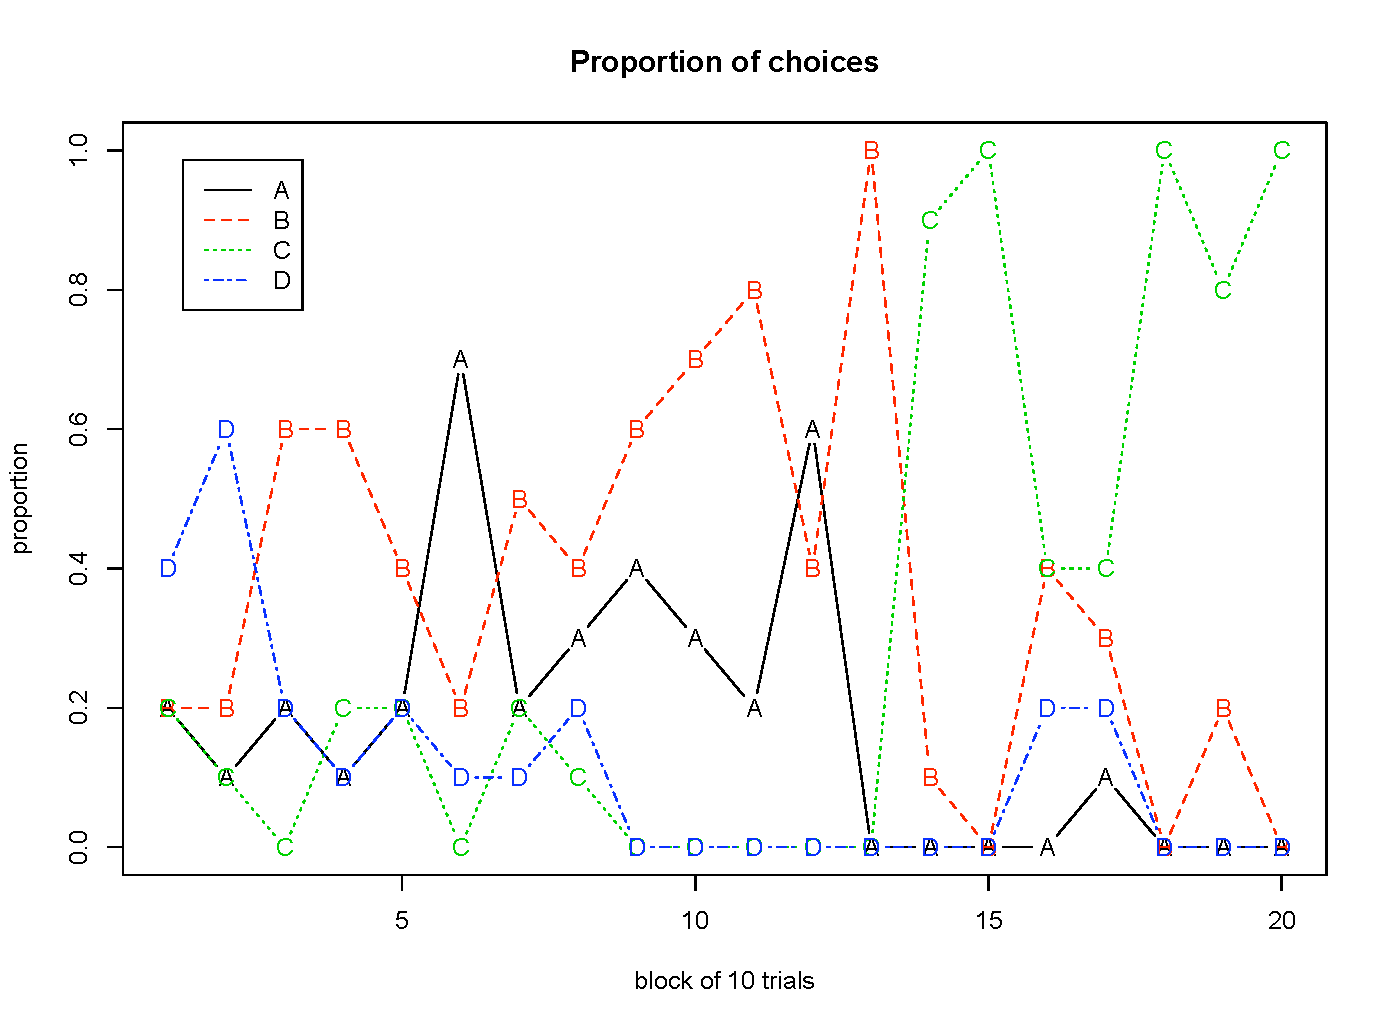
\includegraphics[width=7cm]{graphs/igtdata4.pdf}

\begin{itemize}
	\item N=200
	\item 4 choice data, displayed in blocks of 20 trials
	\item optimal strategy is choosing C or D
\end{itemize}


Results are the 4-state model (best by AIC/BIC), model predicted 
probabilities are in the figure ???. States are characterized by 
different types of behavior, shifting from B/D strategy to C/D 
(optimal) strategy. 

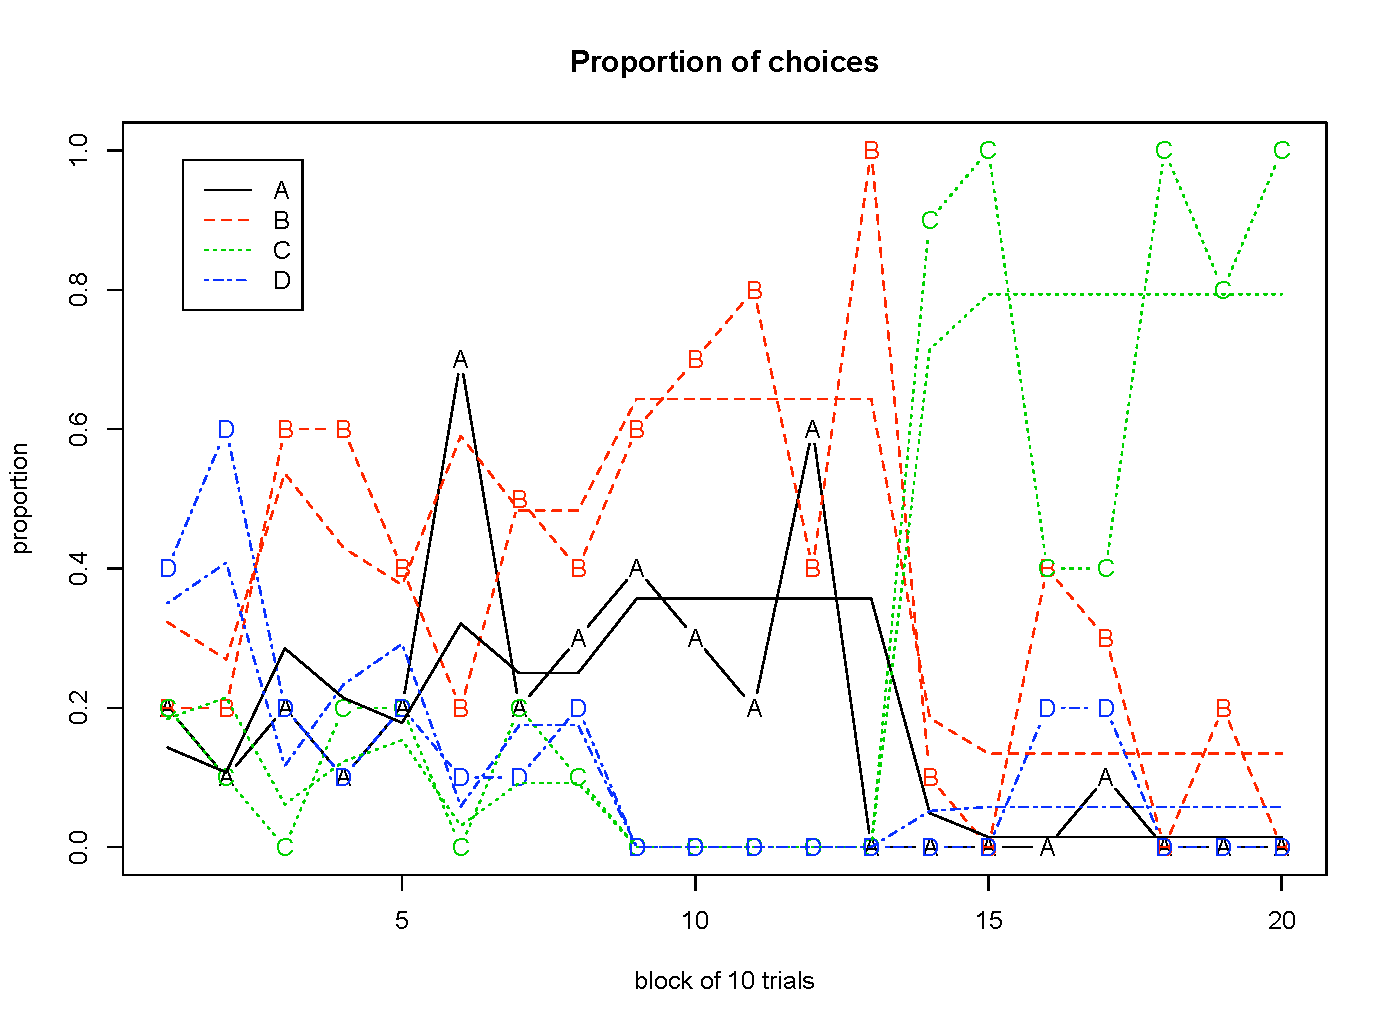
\includegraphics[width=7cm]{graphs/igtmodels4.pdf}
	
	

\subsection{Weather prediction task}

%Still to add models and data. 

The Weather Prediction Task (WPT, Knowlton, Squire \& Gluck, 1994) 
is a probabilistic categorization task, in which participants learn to 
predict the state of the weather (sunny, or rainy) on the basis 
of four ``tarot'' cards (cards with abstract geometrical patterns). 
Each cue pattern is associated with a particular probability distribution 
over the states of the weather. In order to perform in the task, 
participants must predict the weather in accordance with these
conditional probabilities.

%The WPT has been popular in neuropsychological research, 
%particularly because amnesic patients perform this task rather
%well, despite not being able to remember actually many aspects
%of the task (or in some cases, even performing the task at all).
%This has led to the conclusion that probabilistic category learning
%depends on implicit memory, which is separate from explicit
%memory. While this conclusion is debatable (Speekenbrink, Channon 
%\& Shanks, 2008), the finding of relatively unimpaired performance
%by amnesic individuals remains striking.

There are different accounts of probabilistic category learning. 
According to instance or exemplar learning theories, participants
learn by storing each encountered cue-outcome pairing. When presented
with a cue pattern, these exemplars are retrieved from memory, and weighted
according to their similarity to the probe cue pattern, to form a 
classification. According to associative theories, participants gradually 
learn by gradually associating the individual cues (or cue patterns in 
configural learning) to the outcomes. In rule-learning, participants are 
taken to extract rules by which to categorize the different cue patterns. 
Gluck, Shohamy and Myers (2002) proposed a number of such rules (or strategies). A main
difference between these is whether responses are based on the 
presence/absence of a single cue, or whether responses are based on 
cue patterns. Gluck et al. formulated all strategies in a deterministic and
optimal manner (e.g., the multi-cue strategy corresponded to giving the optimal
response to each cue pattern). Meeter et al. allowed for probabilistic 
responding (a small probability of giving the non-optimal response). 

Alternative non-strategy based analyses of the WPT (Lagnado et al, Speekenbrink et al) 
have estimated response strategies by logistic regression, allowing the regression
coefficients to change over time.  

%associative, rule-based.  
Here, we analyze the behavior of a single individual performing the
WPT for 200 trials. We chose to analyse the ``average'' participant (the
participant with performance closest to the group average) in a large
unpublished dataset. We let each state be characterized by a GLM with a 
Binomial distributed response and logistic link function (i.e., a logistic
regression model). We are particularly interested in evidence for 
strategy switching and whether a DMM can recover a strategy model 
in line with Gluck et al. (2002). 

As we fit the data to a single subject, 
we must place some constraints. Specifically, we constrain the state 
transitions to be in a ``left-right'' format (states can only proceed 
to the immediately adjacent state and never back, and must start in 
the initial state). We fitted a single, two and three state model to 
the data. This showed that a two state model was better than a single
and three state model.

\begin{table}
\caption{Estimates for the weather prediction task}
\label{tab:WPT}
\begin{tabular}{lcccccccc} \hline
 & & \multicolumn{1}{c}{1 state} & & \multicolumn{2}{c}{2 state} && \multicolumn{2}{c}{2 state (constr.)} \\ \cline{3-3} \cline{5-6} \cline{8-9}
parameter & & $S_1$ & & $S_1$ & $S_2$ & & $S_1$ & $S_2$ \\ \hline
(intercept) & & -0.69 & & -2.73 & 0.88 & & -1.24 & 0 \\
cue 1 && 1.69 && 2.12 & 1.60 && 1.65 & 1.97 \\
cue 2 && 1.12 && 0.97 & 1.63 && 0 & 1.92 \\
cue 3 && -0.49 && 0.91 & -2.03 && 0 & -1.58 \\
cue 4 && -1.32 && 0.69 & -3.16 && 0 & -2.67 \\ \hline
 & & \multicolumn{1}{c}{AIC=204.47} & & \multicolumn{2}{c}{AIC=187.50} && \multicolumn{2}{c}{AIC=185.24}
\end{tabular}
\end{table}

Investigation of the parameter estimates (see Table~\ref{tab:WPT}) indicated that the first state might be
a single cue strategy (the regression coefficient for the first cue was of much 
larger magnitude than that of the other cues). The second state was a multi-cue
strategy (all cues had regression coefficients of reasonable magnitude). 
To reduce the degrees of freedom, and improve parameter estimates, we implemented 
constraints to force state 1 into a single cue strategy (fixing the coefficients
of the remaining three cues to 0) and state 2 in a multi-cue strategy (forcing
the intercept to 0). These restrictions resulted in a better AIC value of AIC=185.24 
(df=7). Interestingly, the single cue strategy was somewhat different than 
described by Gluck et al. Parameter estimates indicated relatively more consistent 
predictions of ``rain'' in the absence of cue 1 ($Pr(\text{sun}) = 0.22$) and more
inconsistent predictions of ``sun'' in the presence of cue 1 ($Pr(\text{sun}) = 0.60$). 
The cue weights of the multi-cue strategy were in the direction of the optimal weights. 
The Viterbi state sequence indicated that the participant used the single
cue strategy for the first 60 trials, and then switched to the multi-cue strategy.

\section{Discussion}
	
\begin{itemize}
	\item depmixS4 can be downloaded from: http://r-forge.r-project.org/depmix/
	\item It is feasible to fit hidden Markov models in moderate length time series
	\item Many applications in experimental psychology
	\item Future developments: 
	\begin{enumerate}
		\item richer measurement models, eg factor models, AR models etc
		\item richer transition models, eg continuous time measurement occasions
		\item explicit state durations
		\item identifiability of models
		\item model selection
	\end{enumerate}
	\item standard errors of parameters
\end{itemize}



References

Bechara, A., Damasio, A. R., Damasio, H., \& Anderson, S. W.(1994).
Insensitivity to future consequences following damage to human
prefrontal cortex.  Cognition, 50(1�3), 7�15.

Chambers, J. M. (1998). Programming with Data: A Guide to the S Lan-
guage. New York: Springer-Verlag.

Crone, E. A.,  \& van der Molen, M. W. (2004).  Developmental changes in
real life decision making: Performance on a gambling task previously
shown to depend on the ventromedial prefrontal cortex.  Developmental
Neuropsychology, 25(3), 251-279.

Dunn, B. D., Dalgleish, T.,  \& Lawrence, A. D. (2006).  The somatic
marker hypothesis: A critical evaluation.  Neuroscience and
Biobehavioral Reviews, 30(2), 239-271.

Gluck, M. A., Shohamy, D., \& Myers, C. (2002). How do people solve the 
weather prediction task?: Individual variability in strategies for 
probabilistic category learning. Learning \& Memory, 9, 408-418.

Huizenga, H. M., Crone, E. A., \& Jansen, B. R. J. (2007).
Decision-making in healthy children, adolescents and adults explained
by the use of increasingly complex proportional reasoning rules.
Developmental Science, 10(6), 814-825.

Knowlton, B. J., Squire, L. R., \& Gluck, M. A. (1994). 
Probabilistic classification learning in amnesia. 
Learning \& Memory, 1 , 106-120.

Siegler, R. S. (1981).  Developmental sequences within and between
concepts.  Monographs of the Society for Research in Child
Development, 46(2, Serial No.  189).

Visser, Raijmakers, \& Van der Maas (2008). Dynamics book chapter. 

\section*{Author note}

Ingmar Visser was supported by an EC Framework 6 grant, project 516542
(NEST).  Maarten Speekenbrink was supported by the ESRC Centre for
Economic Learning and Social Evolution (ELSE).  Thanks to Hilde
Huizenga, Brenda Jansen and Anna van Duijvenvoorde for the Iowa
Gambling task data and David Lagnado for the Weather Prediction Task
data.


\bibliography{all,ingmar}


\end{document}















